\documentclass{article}

\usepackage{amsmath}
\usepackage{amsfonts}
\usepackage{subcaption}
\usepackage{booktabs}
\usepackage{hyperref}
\usepackage{placeins}
\usepackage[]{algorithm2e}
\usepackage{tabularx}
\usepackage{makecell}

\usepackage{graphicx}
\usepackage{pgfplots}
\pgfplotsset{
        table/search path={data},
    }
\pgfplotsset{compat=newest}
\usepackage{tikz}

\usepackage{geometry}
 \geometry{
 a4paper,
 total={170mm,257mm},
 left=20mm,
 top=20mm,
 }

\begin{document}
	\title{Continual Learning Project}
	
	\author{Term 1 Update}
	
	\maketitle

\section{Latest Experiments}
    
From our most recent discussions, the experiments I ran focused on looking 
at the way in which the generalisation error and rate of forgetting between 
the two teachers varied with the amount of overlap between different layers. 

There is a lot to unpack so I highlight one observation in the plots below. 
I have added the raw tensorboard logs to the google drive here:\\ 

\href{https://drive.google.com/drive/folders/1SDVxsGVrHZesUncODQXMhKiUPnOCzW3p}{https://drive.google.com/drive/folders/1SDVxsGVrHZesUncODQXMhKiUPnOCzW3p}\\

\noindent if you want to look in more detail. 

\subsection{Periodic - ReLU}

In this setup the teacher is changed with a fixed period of 5000 training steps. 
I ran the experiment with five different random seeds. This section shows results with the ReLU non-linearity.

\subsubsection{Independent Teachers}

\begin{figure}[htpb]
    \centering
    \pgfplotsset{
        width=0.8\textwidth,
        height=0.6\textwidth,
        legend style={at={(axis cs:-0.5,-1)},anchor=south west},
    % 	legend style={at={(0.97,0.03)},
    % 		anchor=south east},
        label style={font=\large},
        legend cell align = {left},
        xmin=0, xmax=1,
        ymin=0, ymax=1,
        cycle list={
    % 	{red, densely dotted, ultra thick},
    % 	{blue, solid, thick},
    % 	{black!45!green, loosely dashed, ultra thick},
    % 	{yellow, loosely dotted, ultra thick},
        {green!45!black, thick},
        {red, thick},
        {orange, thick},
        {blue, thick},
        {red!45!blue, thick}}}
    \begin{tikzpicture}
    \begin{axis}
    [
        scaled x ticks = true,
        xlabel={\small Training steps},
        % ylabel={\small Meta validation loss, $\Delta_{\text{Test}}$},
        ylabel={\small Generalisation Error (log)},
        xtick={0,0.5,1},
        xtick distance=0.5,
        xticklabels={0, 50000, 100000},
        ytick distance=0.25,
        % ytick={0,0.12,0.24, 0.36, 0.48,0.6,0.72,0.84, 0.96},
        yticklabels={-20, -16, -12, -8, -4, 0},
        legend pos=south east,
        % xmajorgrids=true,
        % ymajorgrids=true,
        % grid style=dashed,
    ]
    \addplot graphics [xmin=0,xmax=1,ymin=0,ymax=1] {independent_seed_5_full.png};
    \end{axis}
    \end{tikzpicture}%
    \vspace{0.2em}
    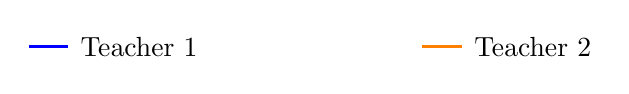
\begin{tikzpicture}
    % 	\draw (-3.2,-0.5) -- (-3.2,0.3) -- (1.6,0.3) -- (1.6,-0.5) -- (-3.2,-0.5);
        \draw [blue, thick] (-9,-0.2) -- (-8.5,-0.2);
        \node at (-7.6, -0.2) {Teacher 1};
        \draw [orange, thick] (-4,-0.2) -- (-3.5,-0.2);
        \node at (-2.6, -0.2) {Teacher 2};
    \end{tikzpicture}
    % \vspace{1em}
    \caption[]{At the start of training, the rate of forgetting is very large.
    Very quickly however this levels off and performance on the network not currently
    being used to train the student stays level.}\label{fig: results17}
\end{figure}
\FloatBarrier

\newpage

\subsubsection{Overlap 25-50\%}

\begin{figure}[htpb]
    \centering
    \pgfplotsset{
        width=0.46\textwidth,
        height=0.38\textwidth,
        legend style={at={(axis cs:-0.5,-1)},anchor=south west},
    % 	legend style={at={(0.97,0.03)},
    % 		anchor=south east},
        label style={font=\large},
        legend cell align = {left},
        xmin=0, xmax=1,
        ymin=0, ymax=1,
        cycle list={
    % 	{red, densely dotted, ultra thick},
    % 	{blue, solid, thick},
    % 	{black!45!green, loosely dashed, ultra thick},
    % 	{yellow, loosely dotted, ultra thick},
        {green!45!black, thick},
        {red, thick},
        {orange, thick},
        {blue, thick},
        {red!45!blue, thick}}}
        \begin{tikzpicture}
            \begin{axis}
            [
                scaled x ticks = true,
                scaled y ticks = true,
                xlabel={\small Training steps},
                % ylabel={\small Meta validation loss, $\Delta_{\text{Test}}$},
                ylabel={\small Generalisation Error (log)},
                xtick={0,0.5,1},
                xtick distance=0.5,
                xticklabels={0, 50000, 100000},
                ytick distance=0.25,
                % ytick={0,0.12,0.24, 0.36, 0.48,0.6,0.72,0.84, 0.96},
                yticklabels={-20, -16, -12, -8, -4, 0},
                legend pos=south east,
                % xmajorgrids=true,
                % ymajorgrids=true,
                % grid style=dashed,
                title={25\% Overlap}
            ]
            \addplot graphics [xmin=0,xmax=1,ymin=0,ymax=1] {overlap25_seed_5_full.png};
            % \addplot + table [y=reward, x=step_count, col sep=comma, mark=none] {ppo_learning_curve_lim.csv};\addlegendentry{PPO}
            % \addplot + table [y=reward, x=step_count, col sep=comma, mark=none] {a2c_learning_curve_lim.csv};\addlegendentry{A2C}
            % \addplot + table [y=reward, x=step_count, col sep=comma, mark=none] {ppo_lstm_learning_curve_lim.csv};\addlegendentry{PPO + LSTM}
            % \addplot + table [y=reward, x=step_count, col sep=comma, mark=none] {a2c_lstm_learning_curve_lim.csv};\addlegendentry{A2C + LSTM}
            \end{axis}
            \end{tikzpicture}%
            \vspace{0.2cm}
            \begin{tikzpicture}
            \begin{axis}
            [
                scaled x ticks = true,
                scaled y ticks = true,
                xlabel={\small Training steps},
                ylabel={\small Generalisation Error (log)},
                xtick={0,0.5,1},
                xtick distance=0.5,
                xticklabels={0, 50000, 100000},
                ytick distance=0.25,
                % ytick={0,0.12,0.24, 0.36, 0.48,0.6,0.72,0.84, 0.96},
                yticklabels={-20, -16, -12, -8, -4, 0},
                legend pos=south east,
                % xmajorgrids=true,
                % ymajorgrids=true,
                % grid style=dashed,
                title={50\% Overlap}
            ]
            \addplot graphics [xmin=0,xmax=1,ymin=0,ymax=1] {overlap50_seed_5_full.png};
            \end{axis}
            \end{tikzpicture}%
    \vspace{0.2em}
    % \begin{tikzpicture}
    % % 	\draw (-3.2,-0.5) -- (-3.2,0.3) -- (1.6,0.3) -- (1.6,-0.5) -- (-3.2,-0.5);
    %     \draw [blue, thick] (-9,-0.2) -- (-8.5,-0.2);
    %     \node at (-7.6, -0.2) {Teacher 1};
    %     \draw [orange, thick] (-4,-0.2) -- (-3.5,-0.2);
    %     \node at (-2.6, -0.2) {Teacher 2};
    % \end{tikzpicture}
    % \vspace{1em}
    \caption[]{With 25 and 50\% overlaps they are not clearly distinguishable
    from the independent case although the 50\% case seems to separate itself a little already.
    Oddly it takes longer to stop forgetting than in the independent case.}\label{fig: results16}
\end{figure}
\FloatBarrier

\subsubsection{Overlap 75\%}

\begin{figure}[htpb]
    \centering
    \pgfplotsset{
        width=0.72\textwidth,
        height=0.5\textwidth,
        legend style={at={(axis cs:-0.5,-1)},anchor=south west},
    % 	legend style={at={(0.97,0.03)},
    % 		anchor=south east},
        label style={font=\large},
        legend cell align = {left},
        xmin=0, xmax=1,
        ymin=0, ymax=1,
        cycle list={
    % 	{red, densely dotted, ultra thick},
    % 	{blue, solid, thick},
    % 	{black!45!green, loosely dashed, ultra thick},
    % 	{yellow, loosely dotted, ultra thick},
        {green!45!black, thick},
        {red, thick},
        {orange, thick},
        {blue, thick},
        {red!45!blue, thick}}}
    \begin{tikzpicture}
    \begin{axis}
    [
        scaled x ticks = true,
        xlabel={\small Training steps},
        % ylabel={\small Meta validation loss, $\Delta_{\text{Test}}$},
        ylabel={\small Generalisation Error (log)},
        xtick={0,0.5,1},
        xtick distance=0.5,
        xticklabels={0, 50000, 100000},
        ytick distance=0.25,
        % ytick={0,0.12,0.24, 0.36, 0.48,0.6,0.72,0.84, 0.96},
        yticklabels={-20, -16, -12, -8, -4, 0},
        legend pos=south east,
        % xmajorgrids=true,
        % ymajorgrids=true,
        % grid style=dashed,
    ]
    \addplot graphics [xmin=0,xmax=1,ymin=0,ymax=1] {overlap75_seed_5_full.png};
    \end{axis}
    \end{tikzpicture}%
    \vspace{0.2em}
    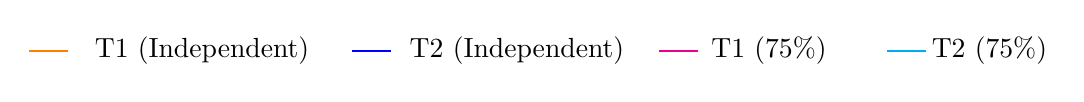
\begin{tikzpicture}
    % 	\draw (-3.2,-0.5) -- (-3.2,0.3) -- (1.6,0.3) -- (1.6,-0.5) -- (-3.2,-0.5);
        \draw [orange, thick] (-12,-0.2) -- (-11.5,-0.2);
        \node at (-9.8, -0.2) {T1 (Independent)};
        \draw [blue, thick] (-7.9,-0.2) -- (-7.4,-0.2);
        \node at (-5.8, -0.2) {T2 (Independent)};
        \draw [magenta, thick] (-4,-0.2) -- (-3.5,-0.2);
        \node at (-2.6, -0.2) {T1 (75\%)};
        \draw [cyan, thick] (-1.1,-0.2) -- (-0.6,-0.2);
        \node at (0.2, -0.2) {T2 (75\%)};
        % \draw [blue, thick] (-12,-0.2) -- (-11.5,-0.2);
        % \node at (-10.8, -0.2) {Vanilla};
        % \draw [red!45!blue, thick] (-9,-0.2) -- (-8.5,-0.2);
        % \node at (-7.8, -0.2) {Greedy};
        % \draw [orange, thick] (-6.7,-0.2) -- (-6.2,-0.2);
        % \node at (-5.4, -0.2) {Weighted};
        % \draw [green!45!black, thick] (-4,-0.2) -- (-3.5,-0.2);
        % \node at (-2.6, -0.2) {Importance};
        % \draw [red, thick] (-1.1,-0.2) -- (-0.6,-0.2);
        % \node at (-0.1, -0.2) {Delta};
    \end{tikzpicture}
    \vspace{1em}
    \caption[]{Once we reach 75\% there is a clear split from the independent case.
    There is some co-learning happening but again it starts to take longer to level out
    when teachers are swapped.}\label{fig: results15}
\end{figure}
\FloatBarrier

\newpage

\subsubsection{Overlap 100\%}

\begin{figure}[htpb]
    \centering
    \pgfplotsset{
        width=0.8\textwidth,
        height=0.45\textwidth,
        legend style={at={(axis cs:-0.5,-1)},anchor=south west},
    % 	legend style={at={(0.97,0.03)},
    % 		anchor=south east},
        label style={font=\large},
        legend cell align = {left},
        xmin=0, xmax=1,
        ymin=0, ymax=1,
        cycle list={
    % 	{red, densely dotted, ultra thick},
    % 	{blue, solid, thick},
    % 	{black!45!green, loosely dashed, ultra thick},
    % 	{yellow, loosely dotted, ultra thick},
        {green!45!black, thick},
        {red, thick},
        {orange, thick},
        {blue, thick},
        {red!45!blue, thick}}}
    \begin{tikzpicture}
    \begin{axis}
    [
        scaled x ticks = true,
        xlabel={\small Training steps},
        % ylabel={\small Meta validation loss, $\Delta_{\text{Test}}$},
        ylabel={\small Generalisation Error (log)},
        xtick={0,0.5,1},
        xtick distance=0.5,
        xticklabels={0, 50000, 100000},
        ytick distance=0.25,
        % ytick={0,0.12,0.24, 0.36, 0.48,0.6,0.72,0.84, 0.96},
        yticklabels={-20, -16, -12, -8, -4, 0},
        legend pos=south east,
        % xmajorgrids=true,
        % ymajorgrids=true,
        % grid style=dashed,
    ]
    \addplot graphics [xmin=0,xmax=1,ymin=0,ymax=1] {overlap100_seed_5_full2.png};
    \end{axis}
    \end{tikzpicture}%
    \vspace{0.2em}
    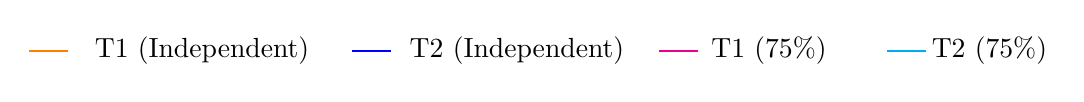
\begin{tikzpicture}
        \draw [orange, thick] (-12,-0.2) -- (-11.5,-0.2);
        \node at (-9.8, -0.2) {T1 (Independent)};
        \draw [blue, thick] (-7.9,-0.2) -- (-7.4,-0.2);
        \node at (-5.8, -0.2) {T2 (Independent)};
        \draw [magenta, thick] (-4,-0.2) -- (-3.5,-0.2);
        \node at (-2.6, -0.2) {T1 (75\%)};
        \draw [cyan, thick] (-1.1,-0.2) -- (-0.6,-0.2);
        \node at (0.2, -0.2) {T2 (75\%)};
    \end{tikzpicture}
    % \vspace{1em}
    \caption[]{There is a strange phenomenon when the overlap reaches the limit of 100\%, which
    is already hinted at above. While there is no discernible forgetting the overall learning 
    is much slower and saturates.}\label{fig: results14}
\end{figure}
\FloatBarrier

This phenomenon of saturation with 100\% overlap of hidden weights holds for all the random seeds I tested:

\begin{figure}[h]
    \centering
    \pgfplotsset{
        width=0.4\textwidth,
        height=0.3\textwidth,
        legend style={at={(axis cs:-0.5,-1)},anchor=south west},
    % 	legend style={at={(0.97,0.03)},
    % 		anchor=south east},
        label style={font=\large},
        legend cell align = {left},
        xmin=0, xmax=1,
        ymin=0, ymax=1,
        cycle list={
    % 	{red, densely dotted, ultra thick},
    % 	{blue, solid, thick},
    % 	{black!45!green, loosely dashed, ultra thick},
    % 	{yellow, loosely dotted, ultra thick},
        {green!45!black, thick},
        {red, thick},
        {orange, thick},
        {blue, thick},
        {red!45!blue, thick}}}
    \begin{tikzpicture}
    \begin{axis}
    [
        scaled x ticks = true,
        scaled y ticks = true,
        xlabel={\small Training steps},
        % ylabel={\small Meta validation loss, $\Delta_{\text{Test}}$},
        ylabel={\small Generalisation Error (log)},
        xtick={0,0.5,1},
        xtick distance=0.5,
        xticklabels={0, 50000, 100000},
        ytick distance=0.25,
        % ytick={0,0.12,0.24, 0.36, 0.48,0.6,0.72,0.84, 0.96},
        yticklabels={-20, -16, -12, -8, -4, 0},
        legend pos=south east,
        % xmajorgrids=true,
        % ymajorgrids=true,
        % grid style=dashed,
    ]
    \addplot graphics [xmin=0,xmax=1,ymin=0,ymax=1] {overlap100_seed_10_full.png};
    % \addplot + table [y=reward, x=step_count, col sep=comma, mark=none] {ppo_learning_curve_lim.csv};\addlegendentry{PPO}
    % \addplot + table [y=reward, x=step_count, col sep=comma, mark=none] {a2c_learning_curve_lim.csv};\addlegendentry{A2C}
    % \addplot + table [y=reward, x=step_count, col sep=comma, mark=none] {ppo_lstm_learning_curve_lim.csv};\addlegendentry{PPO + LSTM}
    % \addplot + table [y=reward, x=step_count, col sep=comma, mark=none] {a2c_lstm_learning_curve_lim.csv};\addlegendentry{A2C + LSTM}
    \end{axis}
    \end{tikzpicture}%
    \vspace{0.2cm}
    \begin{tikzpicture}
    \begin{axis}
    [
        scaled x ticks = true,
        scaled y ticks = true,
        xlabel={\small Training steps},
        ylabel={\small Generalisation Error (log)},
        xtick={0,0.5,1},
        xtick distance=0.5,
        xticklabels={0, 50000, 100000},
        ytick distance=0.25,
        % ytick={0,0.12,0.24, 0.36, 0.48,0.6,0.72,0.84, 0.96},
        yticklabels={-20, -16, -12, -8, -4, 0},
        legend pos=south east,
        % xmajorgrids=true,
        % ymajorgrids=true,
        % grid style=dashed,
    ]
    \addplot graphics [xmin=0,xmax=1,ymin=0,ymax=1] {overlap100_seed_15_full.png};
    \end{axis}
    \end{tikzpicture}%
    \hspace{0.01cm}
    \begin{tikzpicture}
    \begin{axis}
    [
        scaled x ticks = true,
        xlabel={\small Training steps},
        % ylabel={\small Meta validation loss, $\Delta_{\text{Test}}$},
        ylabel={\small Generalisation Error (log)},
        xtick={0,0.5,1},
        xtick distance=0.5,
        xticklabels={0, 50000, 100000},
        ytick distance=0.25,
        % ytick={0,0.12,0.24, 0.36, 0.48,0.6,0.72,0.84, 0.96},
        yticklabels={-20, -16, -12, -8, -4, 0},
        legend pos=south east,
        % xmajorgrids=true,
        % ymajorgrids=true,
        % grid style=dashed,
    ]
    \addplot graphics [xmin=0,xmax=1,ymin=0,ymax=1] {overlap100_seed_20_full2.png};
    % \addplot + table [y=reward, x=step_count, col sep=comma, mark=none] {ppo_learning_curve_lim.csv};\addlegendentry{PPO}
    % \addplot + table [y=reward, x=step_count, col sep=comma, mark=none] {a2c_learning_curve_lim.csv};\addlegendentry{A2C}
    % \addplot + table [y=reward, x=step_count, col sep=comma, mark=none] {ppo_lstm_learning_curve_lim.csv};\addlegendentry{PPO + LSTM}
    % \addplot + table [y=reward, x=step_count, col sep=comma, mark=none] {a2c_lstm_learning_curve_lim.csv};\addlegendentry{A2C + LSTM}
    \end{axis}
    \end{tikzpicture}%
    \vspace{0.2cm}
    \begin{tikzpicture}
    \begin{axis}
    [
        scaled x ticks = true,
        xlabel={\small Training steps},
        ylabel={\small Generalisation Error (log)},
        xtick={0,0.5,1},
        xtick distance=0.5,
        xticklabels={0, 50000, 100000},
        ytick distance=0.25,
        % ytick={0,0.12,0.24, 0.36, 0.48,0.6,0.72,0.84, 0.96},
        yticklabels={-20, -16, -12, -8, -4, 0},
        legend pos=south east,
        % xmajorgrids=true,
        % ymajorgrids=true,
        % grid style=dashed,
    ]
    \addplot graphics [xmin=0,xmax=1,ymin=0,ymax=1] {overlap100_seed_25_full.png};
    % \addplot + coordinates {
    % (0, 0)
    % (0, 1)};\addlegendentry{Vanilla}
    % \addplot + coordinates {
    % (0, 0)
    % (0, 1)};\addlegendentry{Weighted Sample}
    % \addplot + coordinates {
    % (0, 0)
    % (0, 1)};\addlegendentry{Importance Sample}
    % \addplot + coordinates {
    % (0, 0)
    % (0, 1)};\addlegendentry{Greedy Sample}
    % \addplot + coordinates {
    % (0, 0)
    % (0, 1)};\addlegendentry{Delta Sample}
    \end{axis}
    \end{tikzpicture}%
    % \vspace{1em}
    % \caption[]{}\label{fig: results}
    \end{figure}
    \FloatBarrier

\newpage
    
\subsection{Periodic - Sigmoid}

In this setup the teacher is changed with a fixed period of 5000 training steps. 
I ran the experiment with five different random seeds. This section shows results with the Sigmoid non-linearity.
I've only shown the plots for independent and full overlap settings, i.e. the two extremes. Other plots like above
are on the google drive. With the sigmoid non-linearity, there is no proper convergence. 

\subsubsection{Independent Teachers}

\begin{figure}[htpb]
    \centering
    \pgfplotsset{
        width=0.8\textwidth,
        height=0.45\textwidth,
        legend style={at={(axis cs:-0.5,-1)},anchor=south west},
    % 	legend style={at={(0.97,0.03)},
    % 		anchor=south east},
        label style={font=\large},
        legend cell align = {left},
        xmin=0, xmax=1,
        ymin=0, ymax=1,
        cycle list={
    % 	{red, densely dotted, ultra thick},
    % 	{blue, solid, thick},
    % 	{black!45!green, loosely dashed, ultra thick},
    % 	{yellow, loosely dotted, ultra thick},
        {green!45!black, thick},
        {red, thick},
        {orange, thick},
        {blue, thick},
        {red!45!blue, thick}}}
    \begin{tikzpicture}
    \begin{axis}
    [
        scaled x ticks = true,
        xlabel={\small Training steps},
        % ylabel={\small Meta validation loss, $\Delta_{\text{Test}}$},
        ylabel={\small Generalisation Error (log)},
        xtick={0,0.5,1},
        xtick distance=0.5,
        xticklabels={0, 50000, 100000},
        ytick distance=0.2,
        % ytick={0,0.12,0.24, 0.36, 0.48,0.6,0.72,0.84, 0.96},
        yticklabels={-20, -3.6, -3, -2.4, -1.8, -1.2, -0.6},
        legend pos=south east,
        % xmajorgrids=true,
        % ymajorgrids=true,
        % grid style=dashed,
    ]
    \addplot graphics [xmin=0,xmax=1,ymin=0,ymax=1] {independent_seed_5_full_sigmoid.png};
    \end{axis}
    \end{tikzpicture}%
    \vspace{0.2em}
    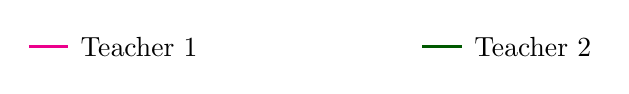
\begin{tikzpicture}
    % 	\draw (-3.2,-0.5) -- (-3.2,0.3) -- (1.6,0.3) -- (1.6,-0.5) -- (-3.2,-0.5);
        \draw [magenta, thick] (-9,-0.2) -- (-8.5,-0.2);
        \node at (-7.6, -0.2) {Teacher 1};
        \draw [green!35!black, thick] (-4,-0.2) -- (-3.5,-0.2);
        \node at (-2.6, -0.2) {Teacher 2};
    \end{tikzpicture}
    % \vspace{1em}
    \caption[]{}\label{fig: results13}
\end{figure}
\FloatBarrier

\subsubsection{Overlap 100\%}

\begin{figure}[htpb]
    \centering
    \pgfplotsset{
        width=0.8\textwidth,
        height=0.45\textwidth,
        legend style={at={(axis cs:-0.5,-1)},anchor=south west},
    % 	legend style={at={(0.97,0.03)},
    % 		anchor=south east},
        label style={font=\large},
        legend cell align = {left},
        xmin=0, xmax=1,
        ymin=0, ymax=1,
        cycle list={
    % 	{red, densely dotted, ultra thick},
    % 	{blue, solid, thick},
    % 	{black!45!green, loosely dashed, ultra thick},
    % 	{yellow, loosely dotted, ultra thick},
        {green!45!black, thick},
        {red, thick},
        {orange, thick},
        {blue, thick},
        {red!45!blue, thick}}}
    \begin{tikzpicture}
    \begin{axis}
    [
        scaled x ticks = true,
        xlabel={\small Training steps},
        % ylabel={\small Meta validation loss, $\Delta_{\text{Test}}$},
        ylabel={\small Generalisation Error (log)},
        xtick={0,0.5,1},
        xtick distance=0.5,
        xticklabels={0, 50000, 100000},
        ytick distance=0.1428,
        % ytick={0,0.12,0.24, 0.36, 0.48,0.6,0.72,0.84, 0.96},
        yticklabels={-20, -4.5, -4, -3.5, -3, -2.5, -2, -1.5, -1, -0.5},
        legend pos=south east,
        % xmajorgrids=true,
        % ymajorgrids=true,
        % grid style=dashed,
    ]
    \addplot graphics [xmin=0,xmax=1,ymin=0,ymax=1] {overlap_100_seed_5_full_sigmoid.png};
    \end{axis}
    \end{tikzpicture}%
    \vspace{0.2em}
    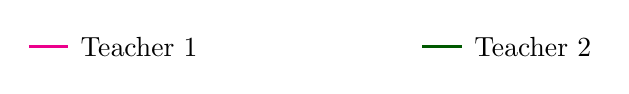
\begin{tikzpicture}
        \draw [magenta, thick] (-9,-0.2) -- (-8.5,-0.2);
        \node at (-7.6, -0.2) {Teacher 1};
        \draw [green!35!black, thick] (-4,-0.2) -- (-3.5,-0.2);
        \node at (-2.6, -0.2) {Teacher 2};
    \end{tikzpicture}
    % \vspace{1em}
    \caption[]{}\label{fig: results1}
\end{figure}
\FloatBarrier

\newpage
    
\subsection{Periodic - Linear}

In this setup the teacher is changed with a fixed period of 5000 training steps. 
I ran the experiment with five different random seeds. This section shows results without a non-linearity.
Again only independent and full overlap shown here. 

\subsubsection{Independent Teachers}

\begin{figure}[htpb]
    \centering
    \pgfplotsset{
        width=0.8\textwidth,
        height=0.45\textwidth,
        legend style={at={(axis cs:-0.5,-1)},anchor=south west},
    % 	legend style={at={(0.97,0.03)},
    % 		anchor=south east},
        label style={font=\large},
        legend cell align = {left},
        xmin=0, xmax=1,
        ymin=0, ymax=1,
        cycle list={
    % 	{red, densely dotted, ultra thick},
    % 	{blue, solid, thick},
    % 	{black!45!green, loosely dashed, ultra thick},
    % 	{yellow, loosely dotted, ultra thick},
        {green!45!black, thick},
        {red, thick},
        {orange, thick},
        {blue, thick},
        {red!45!blue, thick}}}
    \begin{tikzpicture}
    \begin{axis}
    [
        scaled x ticks = true,
        xlabel={\small Training steps},
        % ylabel={\small Meta validation loss, $\Delta_{\text{Test}}$},
        ylabel={\small Generalisation Error (log)},
        xtick={0,0.5,1},
        xtick distance=0.5,
        xticklabels={0, 50000, 100000},
        ytick distance=0.25,
        % ytick={0,0.12,0.24, 0.36, 0.48,0.6,0.72,0.84, 0.96},
        yticklabels={-20, -16, -12, -8, -4, 0, -0.6},
        legend pos=south east,
        % xmajorgrids=true,
        % ymajorgrids=true,
        % grid style=dashed,
    ]
    \addplot graphics [xmin=0,xmax=1,ymin=0,ymax=1] {independent_seed_5_full_linear.png};
    \end{axis}
    \end{tikzpicture}%
    \vspace{0.2em}
    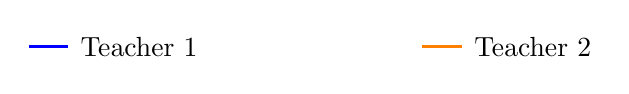
\begin{tikzpicture}
    % 	\draw (-3.2,-0.5) -- (-3.2,0.3) -- (1.6,0.3) -- (1.6,-0.5) -- (-3.2,-0.5);
        \draw [blue, thick] (-9,-0.2) -- (-8.5,-0.2);
        \node at (-7.6, -0.2) {Teacher 1};
        \draw [orange, thick] (-4,-0.2) -- (-3.5,-0.2);
        \node at (-2.6, -0.2) {Teacher 2};
    \end{tikzpicture}
    % \vspace{1em}
    \caption[]{}\label{fig: results17}
\end{figure}
\FloatBarrier

\subsubsection{Overlap 100\%}

\begin{figure}[htpb]
    \centering
    \pgfplotsset{
        width=0.8\textwidth,
        height=0.45\textwidth,
        legend style={at={(axis cs:-0.5,-1)},anchor=south west},
    % 	legend style={at={(0.97,0.03)},
    % 		anchor=south east},
        label style={font=\large},
        legend cell align = {left},
        xmin=0, xmax=1,
        ymin=0, ymax=1,
        cycle list={
    % 	{red, densely dotted, ultra thick},
    % 	{blue, solid, thick},
    % 	{black!45!green, loosely dashed, ultra thick},
    % 	{yellow, loosely dotted, ultra thick},
        {green!45!black, thick},
        {red, thick},
        {orange, thick},
        {blue, thick},
        {red!45!blue, thick}}}
    \begin{tikzpicture}
    \begin{axis}
    [
        scaled x ticks = true,
        xlabel={\small Training steps},
        % ylabel={\small Meta validation loss, $\Delta_{\text{Test}}$},
        ylabel={\small Generalisation Error (log)},
        xtick={0,0.5,1},
        xtick distance=0.5,
        xticklabels={0, 50000, 100000},
        ytick distance=0.25,
        % ytick={0,0.12,0.24, 0.36, 0.48,0.6,0.72,0.84, 0.96},
        yticklabels={-20, -16, -12, -8, -4, 0, -0.6},
        legend pos=south east,
        % xmajorgrids=true,
        % ymajorgrids=true,
        % grid style=dashed,
    ]
    \addplot graphics [xmin=0,xmax=1,ymin=0,ymax=1] {overlap_100_seed_5_full_linear.png};
    \end{axis}
    \end{tikzpicture}%
    \vspace{0.2em}
    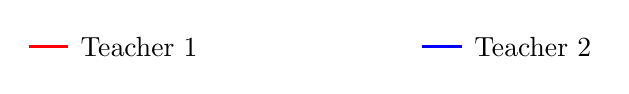
\begin{tikzpicture}
        \draw [red, thick] (-9,-0.2) -- (-8.5,-0.2);
        \node at (-7.6, -0.2) {Teacher 1};
        \draw [blue, thick] (-4,-0.2) -- (-3.5,-0.2);
        \node at (-2.6, -0.2) {Teacher 2};
    \end{tikzpicture}
    % \vspace{1em}
    \caption[]{}\label{fig: results19}
\end{figure}
\FloatBarrier

% \subsection{Fully Interleaved}

% In this setup the teacher is changed after each training step i.e. with period 1. 
% I ran this for five different random seeds.

% In this setting there is not really any discernable forgetting and the two tasks 
% are just learned together. 

\newpage

\section{Experimental Details}

\begin{table}[ht]
    \centering\small
    \caption{Hyperparameters}
        \begin{tabularx}{\linewidth}{lX} 
            \toprule
            Hyperparameter & Value\\
            \midrule
            Optimiser& SGD  \\
            Loss& MSE \\ 
            Non-linearity& ReLU\\
            Teacher Architecture& Input: 500 $\to$ 1 $\to$ 1\\
            Student Architecture& Input: 500 $\to$ 2 $\to$ 1\\
            Learning Rate& 0.2 \\
            Test Batch Size&50000\\
            Train Batch Size& 1   \\
            Teacher Initialisation STD& 1   \\
            Student Initialisation STD& 0.001   \\ 
            Noise& None\\ 
            \bottomrule
    \end{tabularx}
\end{table} 

Currently an overlap of X\% is defined in the following way:
Teacher 1 is randomly initialised. Teacher 2 is initialised such that X\%
of it's hidden weights are exact copies of the corresponding weights in teacher
1, and the rest are also randomly initialised. 

\end{document}